\documentclass{article}

%\usepackage{graphicx}

%\usepackage{amsmath}

\usepackage{gvv-book}

\usepackage{gvv}

%\usepackage{float}

\usepackage{enumitem}

%\usepackage{tfrupee}

%\title{CBSE}

%\usepackage{romannum}

%\date{september 2024}

\begin{document}

\begin{enumerate}
\item If $-5$ is a root of the quadratic equation $2x^2+px-15=0$ and the quadratic equation $p(x^2+x)+k=0$ has equal roots, find the value of $k$.
\end{enumerate}
\end{document}

\item In \figref{fig:circle}, $O$ is the centre of a circle such that diameter $AB
=13 cm$ and $AC=12 cm$. $BC$ is joined. F
ind the area of the shaded region. (Take $\pi=3.14$)
 \begin{figure}[H]
   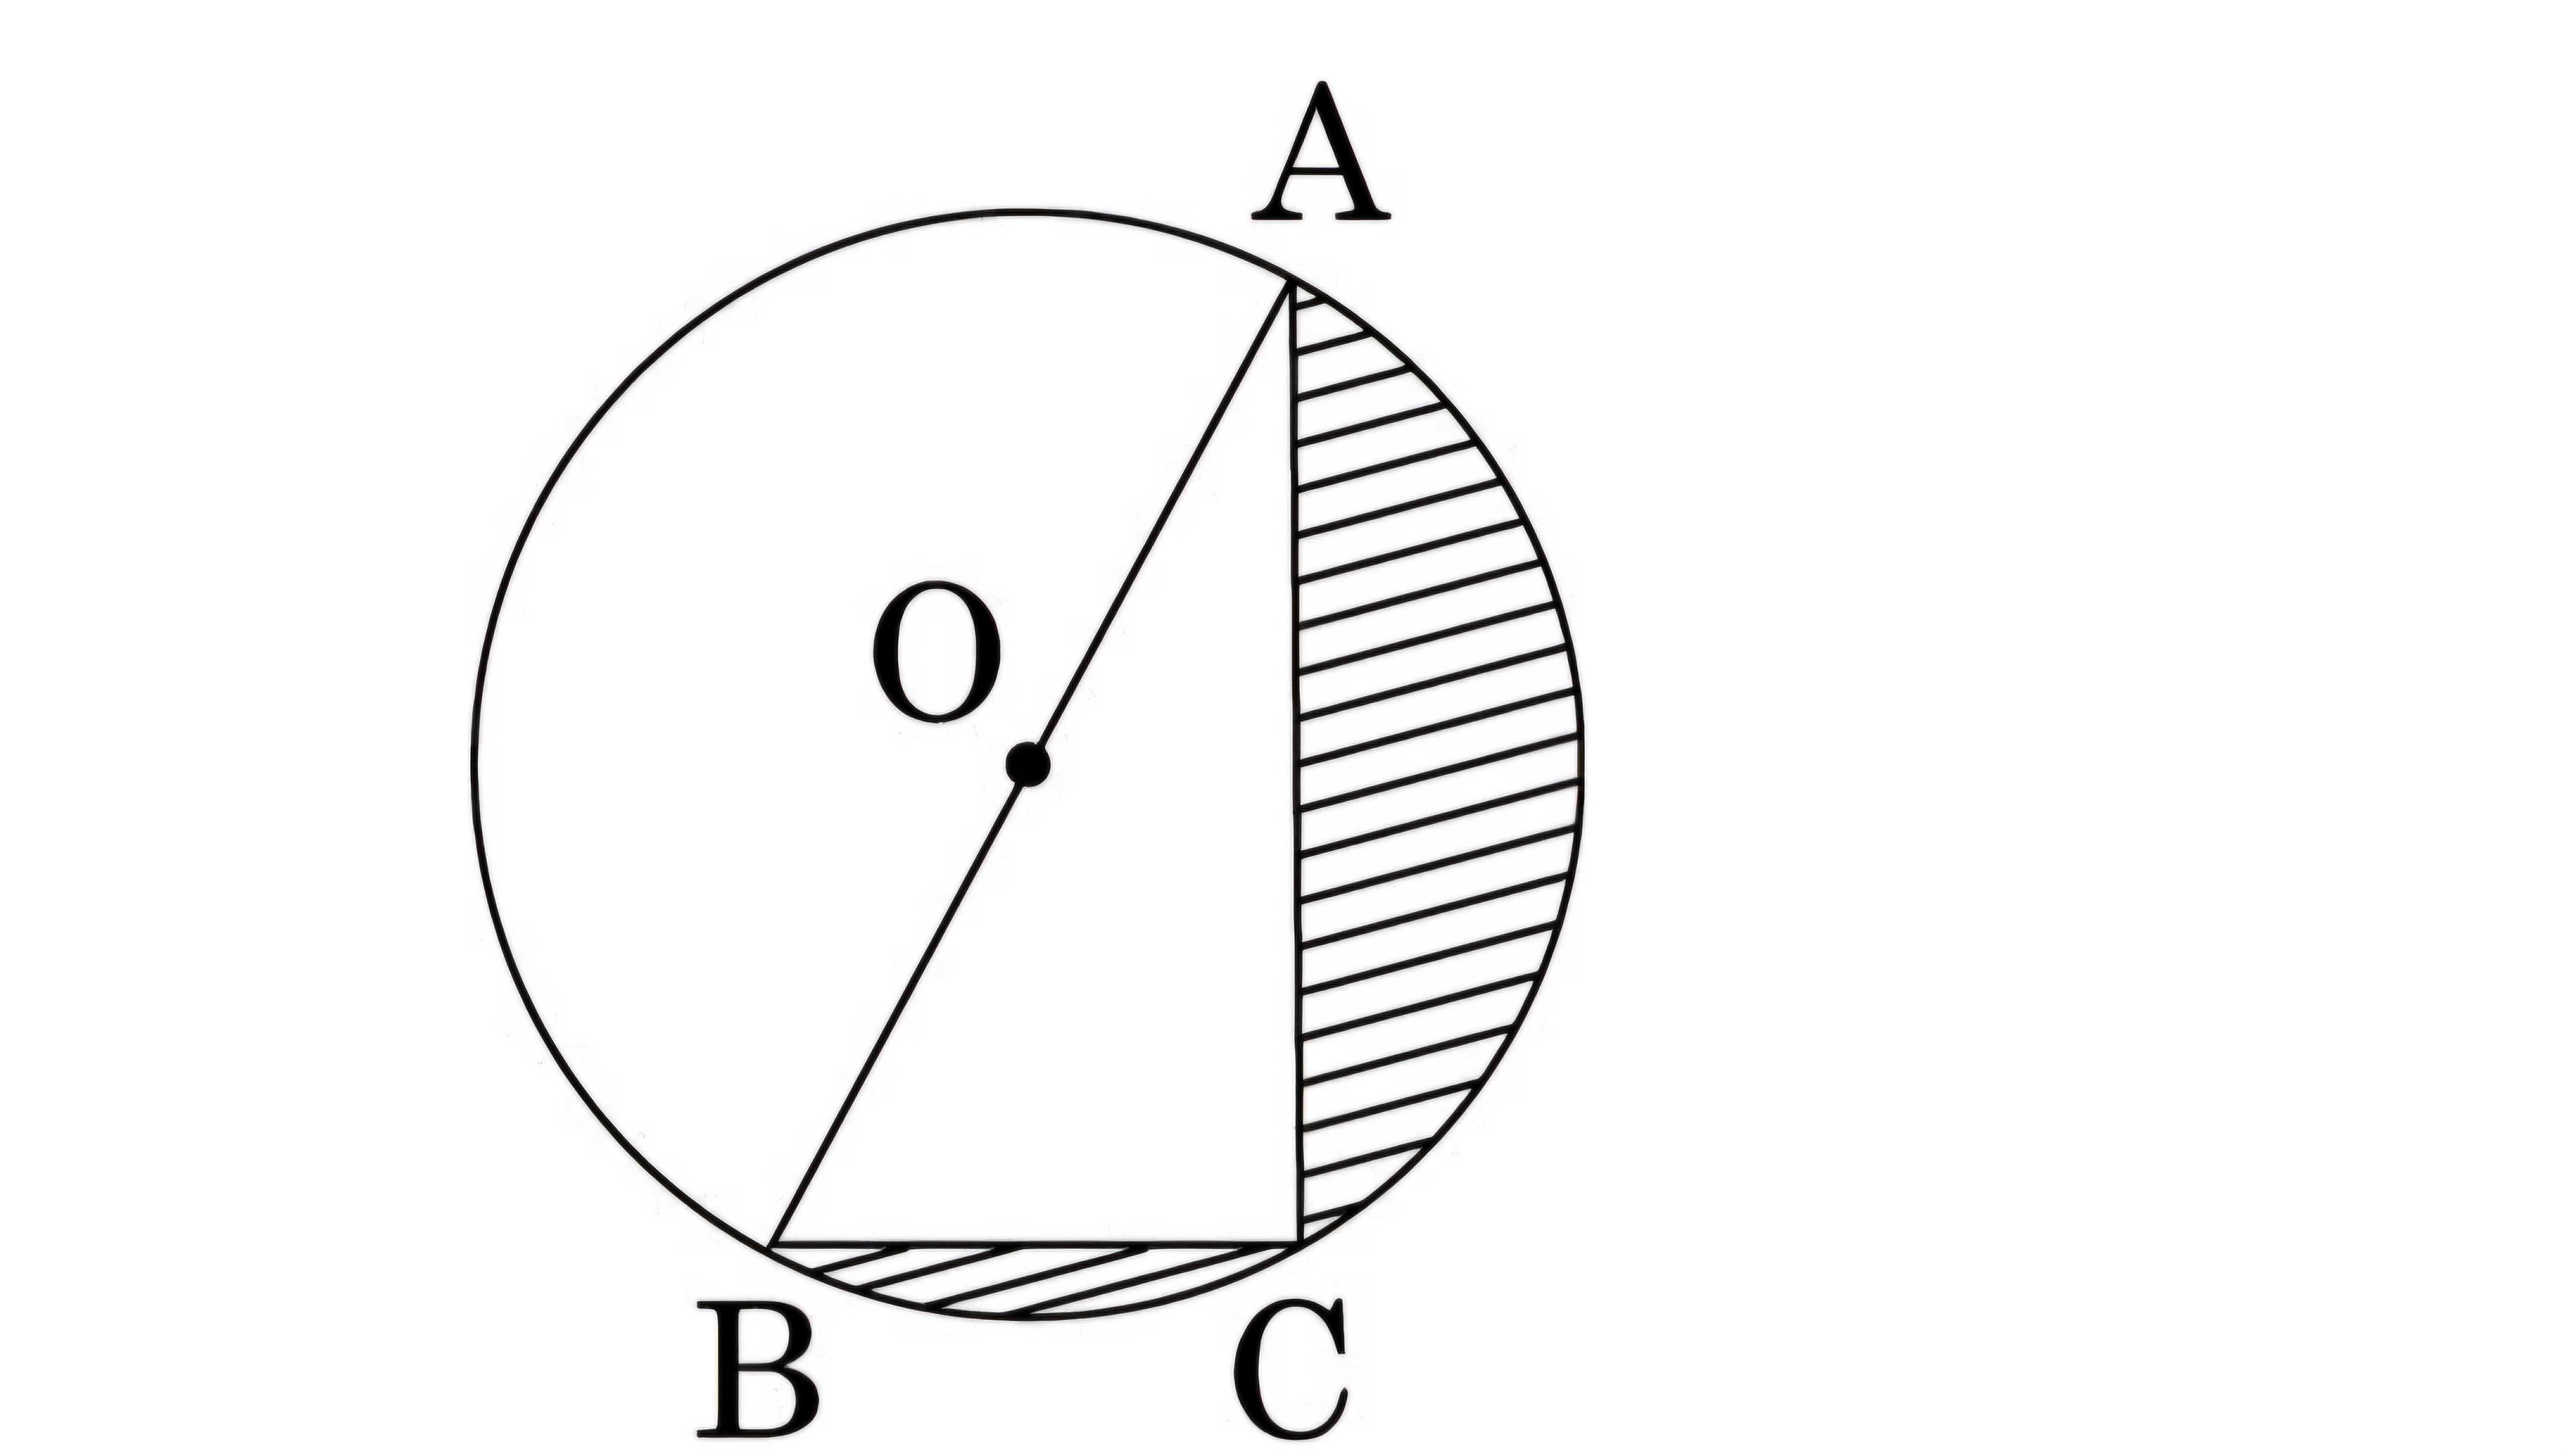
\includegraphics[width=\columnwidth]{.
/figs/circle.jpg}
    \caption{Circle with centre O}
     \label{fig:circle}                        \end{figure}

     \end{enumerate}
     \end{document}

 \item If the ratio of the sum of first $n$ terms of two 5A.P's is $(7n+1):(4n+27)$, find the ratio of their $m^{th}$ terms.   
	 \end{enumerate}
	 \end{document}
 \item solve for $x$:                             \begin{align}                                    \frac{1}{(x-1)(x-2)}+\frac{1}{(x-2)(x-3)}=\frac{2}{3},x \not= 1,2,3                                                \end{align}                      \end{enumerate}
 \end{document}
	\item In \figref{fig:twocircle}, two equal circles,with centres $O$ and $O'$, touch each other at $X$.$OO'$ produced meets
the circle with centre $O'$ at $A$. $AC$
is tangent to the circle with centre $O$, at the point $C$. $O'D$ os perpendicular
 to $AC$. Find the value of $\frac{DO'}{CO}$.                                       \begin{figure}[H]                         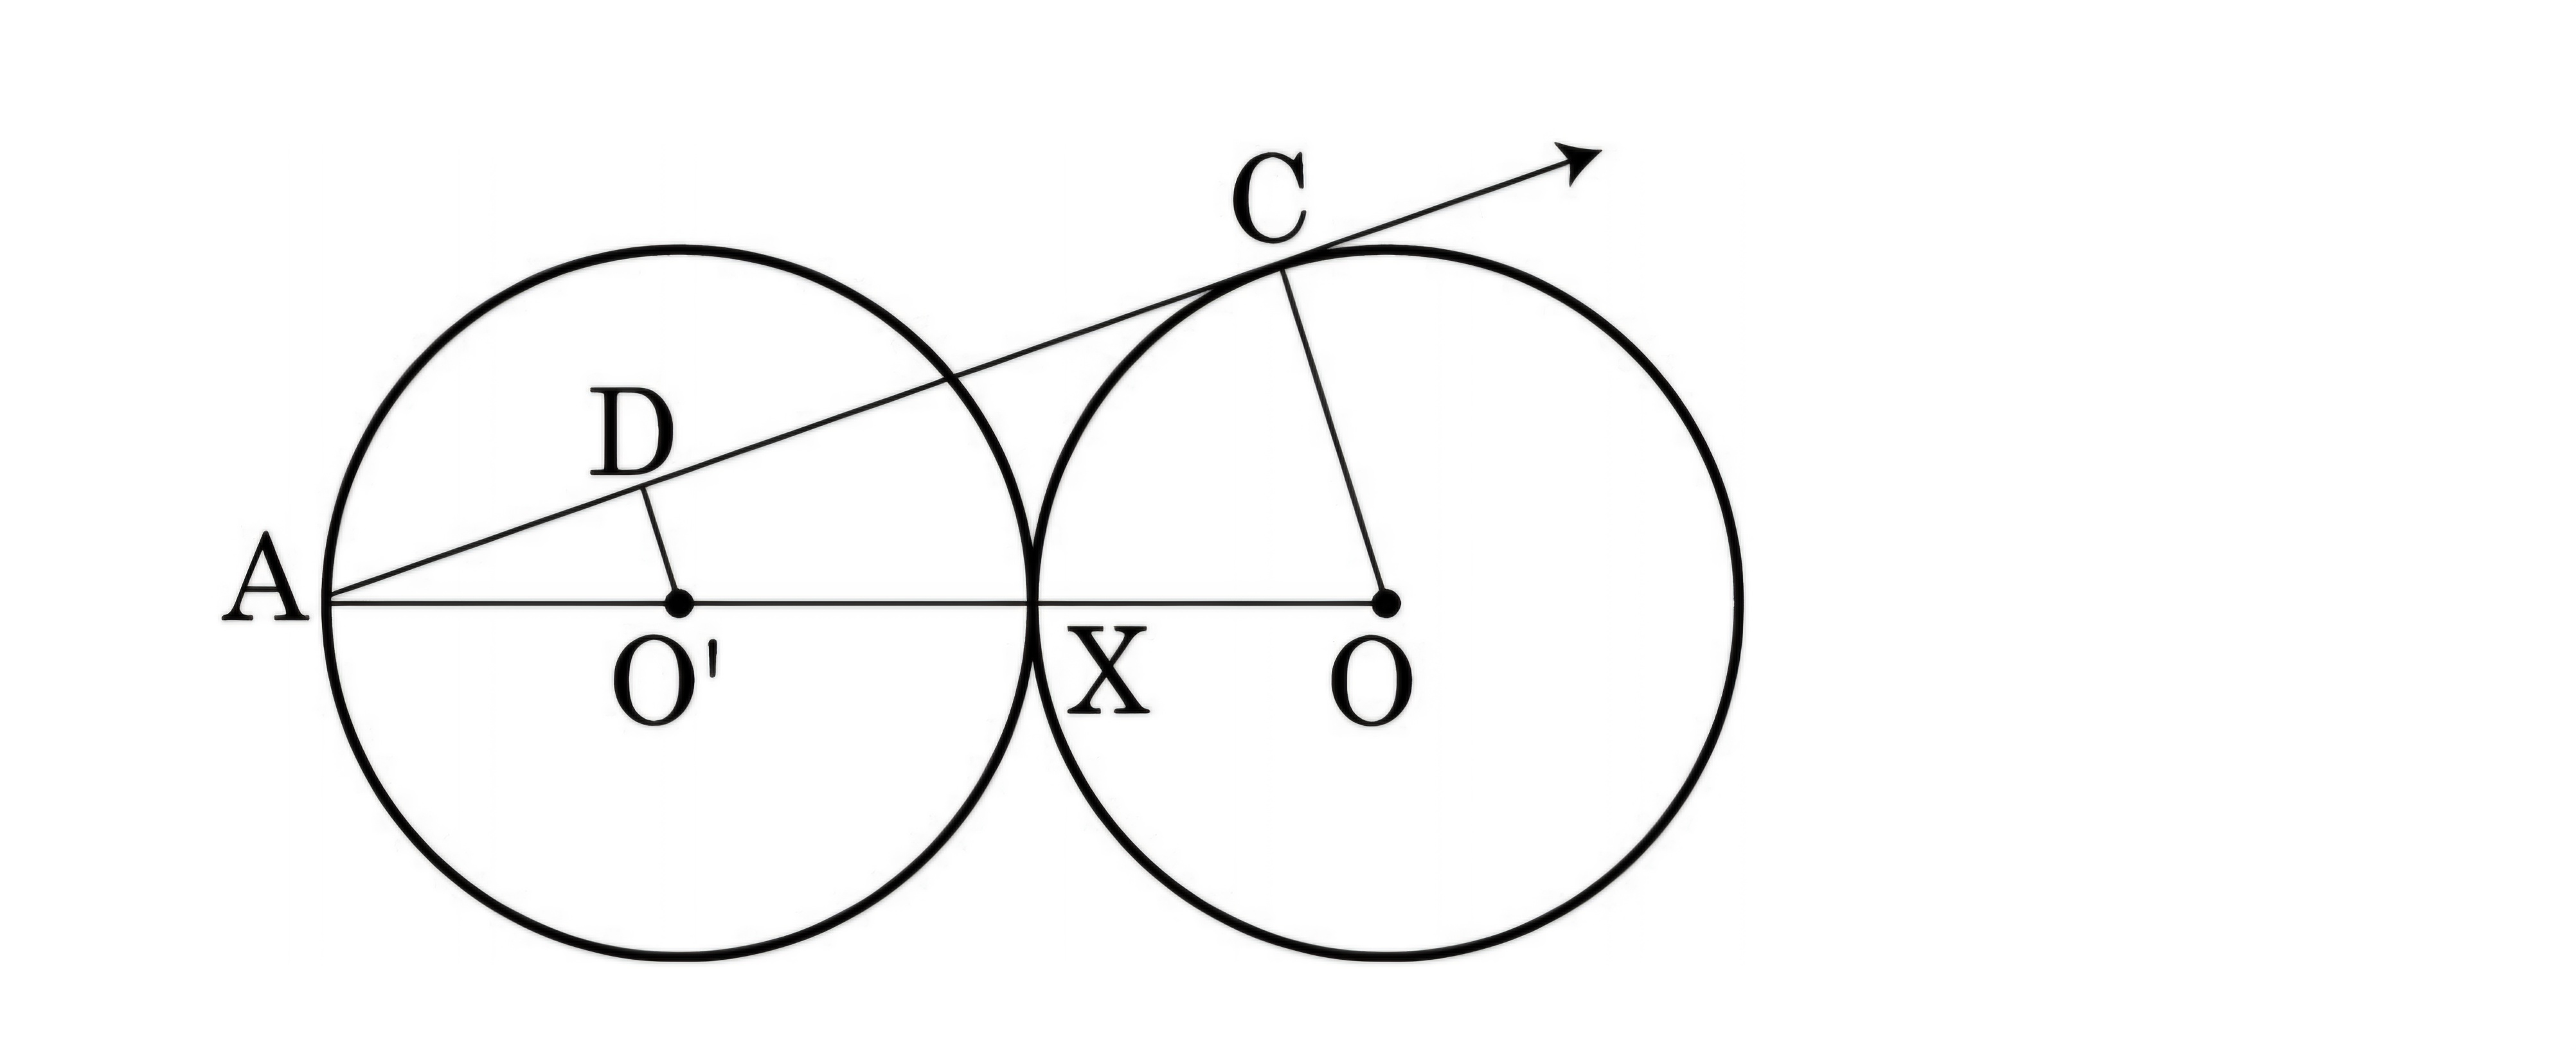
\includegraphics[width=\columnwidth]{./figs/twocircle.jpg}                         \caption{Two equal circles}               \label{fig:twocircle}                    \end{figure}
	 \end{enumerate}
	 \end{document}
